% Section 04: Advanced Sequential Monte Carlo Methods
\section{Advanced Sequential Monte Carlo Methods}

The naive rejection sampling discussed in Section 2 is computationally prohibitive for complex models with high-dimensional summary statistics.
To ensure robust inference, we implemented a Sequential Monte Carlo (SMC) ABC algorithm, which iteratively refines the posterior approximation.

\subsection{SMC-ABC: Efficiency and Adaptive Sampling}

The primary advantage of SMC-ABC is its adaptive sampling efficiency.
Unlike rejection sampling, which suffers from low acceptance rates as the tolerance $\epsilon$ decreases, SMC-ABC maintains a population of $M$ particles that are evolved through a sequence of intermediate distributions \parencite{beaumont2009adaptive, moores2015preprocessing}.
By using an adaptive tolerance schedule—where $\epsilon_t$ is determined by the $\alpha$-th percentile of the previous generation's distances—the algorithm guarantees that we obtain a pre-specified number of samples even at very small tolerances.
The general structure of our implementation is detailed in Algorithm \ref{alg:smc_abc}.

\begin{algorithm}[H]
\caption{Sequential Monte Carlo ABC with Adaptive Tolerance}
\label{alg:smc_abc}
\begin{algorithmic}[1]
    \Require Observed summaries $s_{obs}$, Prior $\pi(\theta)$, Number of particles $M$, Target tolerance $\epsilon_T$
    \Ensure Weighted particles $\{(\theta_i^{(T)}, w_i^{(T)})\}_{i=1}^M$
    
    \State \textbf{Initialization:} Sample $M$ particles $\{\theta_i^{(0)}\}$ from $\pi(\theta)$ and set weights $w_i = 1/M$.
    \For{generation $t = 1$ \textbf{to} $T$}
        \State Set $\epsilon_t$ as the $\alpha$-th percentile of distances from generation $t-1$.
        \State Compute covariance $\Sigma_{t-1}$ of the current population for the perturbation kernel.
        \While{accepted particles $< M$}
            \State Sample $\theta^*$ from $\{\theta_k^{(t-1)}\}$ with weights $w_k^{(t-1)}$.
            \State Perturb $\theta^{**} \sim \mathcal{N}(\theta^*, \Sigma_{t-1})$ using a multivariate normal kernel.
            \State Simulate $y^{**} \sim f(y|\theta^{**})$ and compute $s^{**} = S(y^{**})$.
            \If{$d(s^{**}, s_{obs}) \le \epsilon_t$}
                \State Store $\theta^{**}$ and calculate importance weight $w^{**}$.
            \EndIf
        \EndWhile
        \State Normalize weights $w_i^{(t)}$.
    \EndFor
\end{algorithmic}
\end{algorithm}

\subsection{Comparison of Distance Metrics: Euclidean vs. Mahalanobis}

In our baseline SMC implementation (weighted Euclidean distance), the posterior for $\beta$ and $\rho$ exhibited a strong "ridge," indicating the model's struggle to decouple the two parameters.
By transitioning to the Mahalanobis distance, we accounted for the covariance structure $\mathbf{\Sigma}$ of the 5D summary statistics \parencite{nott2014approximate}:
\begin{equation}
    d(s, s_{obs}) = \sqrt{(s - s_{obs})^T \mathbf{\Sigma}^{-1} (s - s_{obs})}
\end{equation}
As shown in Figure \ref{fig:dist_comparison}, the Mahalanobis metric (b) noticeably reduces the artificial correlation in the posterior compared to the standard approach (a), allowing for a more localized and accurate identification of the true parameter values.

\begin{figure}[H]
    \centering
    \begin{subfigure}[b]{0.48\textwidth}
        \centering
        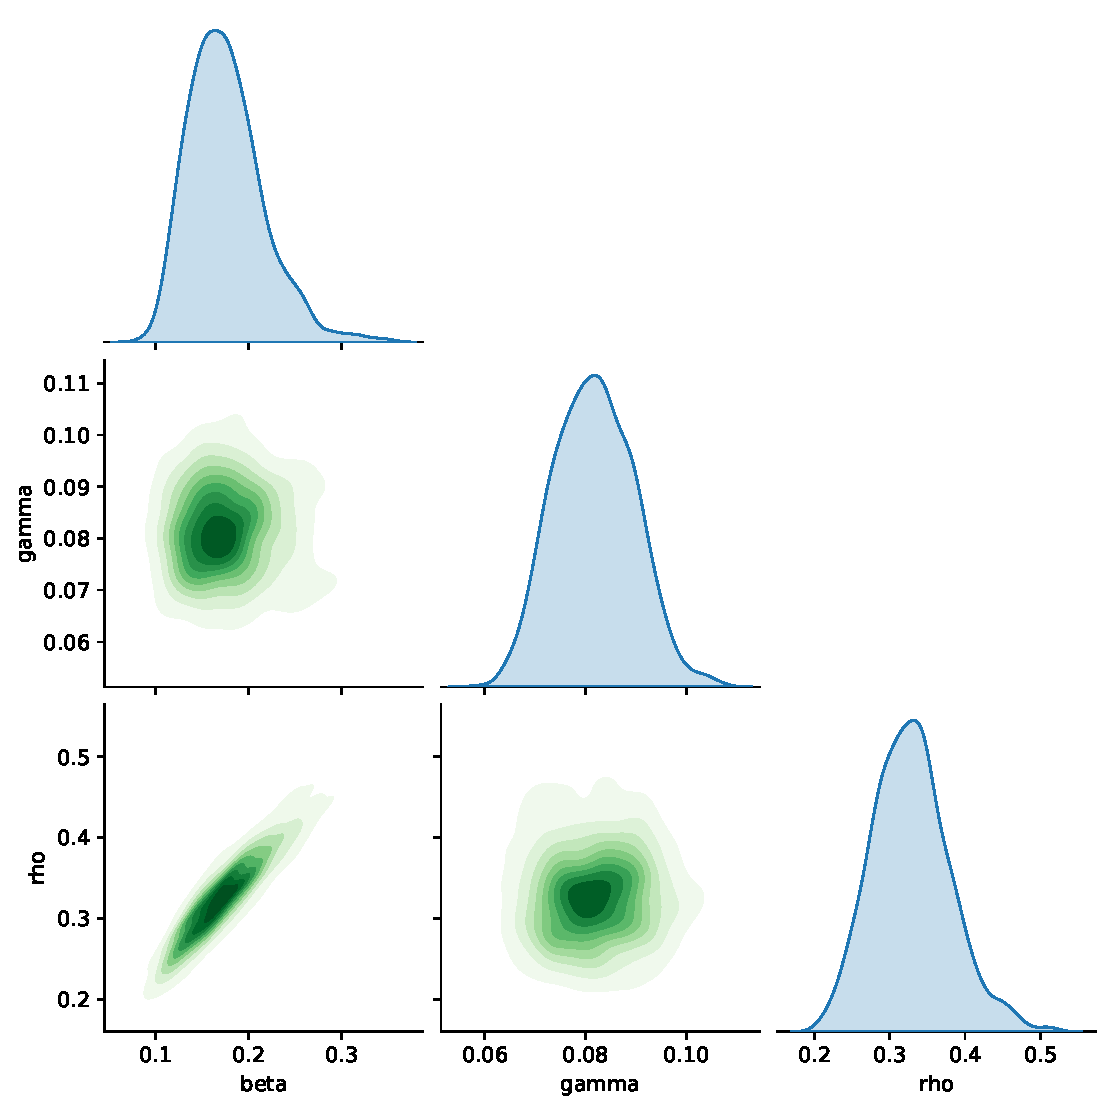
\includegraphics[width=\textwidth]{plots/smc_abc_pairplot_s4_weighted_time.pdf}
        \caption{Weighted Euclidean (Baseline)}
        \label{fig:dist_euclidean}
    \end{subfigure}
    \hfill
    \begin{subfigure}[b]{0.48\textwidth}
        \centering
        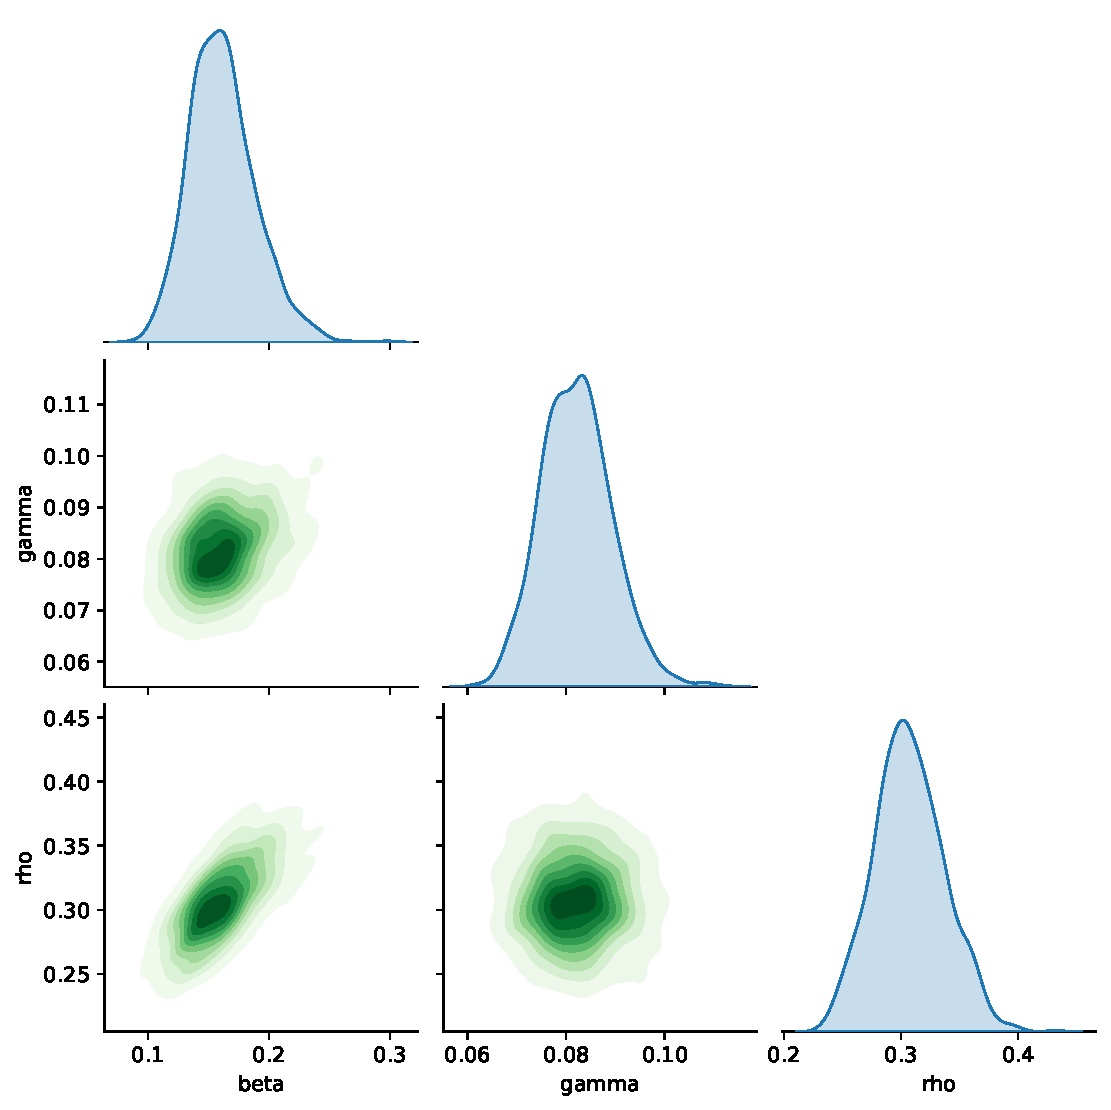
\includegraphics[width=\textwidth]{plots/smc_abc_pairplot_s5_mahalanobis.pdf}
        \caption{Mahalanobis Distance}
        \label{fig:dist_mahalanobis}
    \end{subfigure}
    \caption{Posterior comparison between distance metrics.
The Mahalanobis metric effectively decorrelates the summary statistics, breaking the $\beta$-$\rho$ trade-off ridge.}
    \label{fig:dist_comparison}
\end{figure}

\subsection{Post-processing: Local Linear Regression Adjustment}

To further refine the results and neutralize the bias introduced by a non-zero $\epsilon$, we applied a local linear regression adjustment \parencite{beaumont2002approximate}.
Figure \ref{fig:reg_comparison} illustrates the dramatic "sharpening" effect: the marginal distributions become significantly tighter and more centered around the true values \parencite{blum2017regression}.
Quantitative improvements are summarized in Table \ref{tab:regression_improvement}, showing an average precision gain of approximately 30\%.

\begin{figure}[H]
    \centering
    \begin{subfigure}[b]{0.48\textwidth}
        \centering
        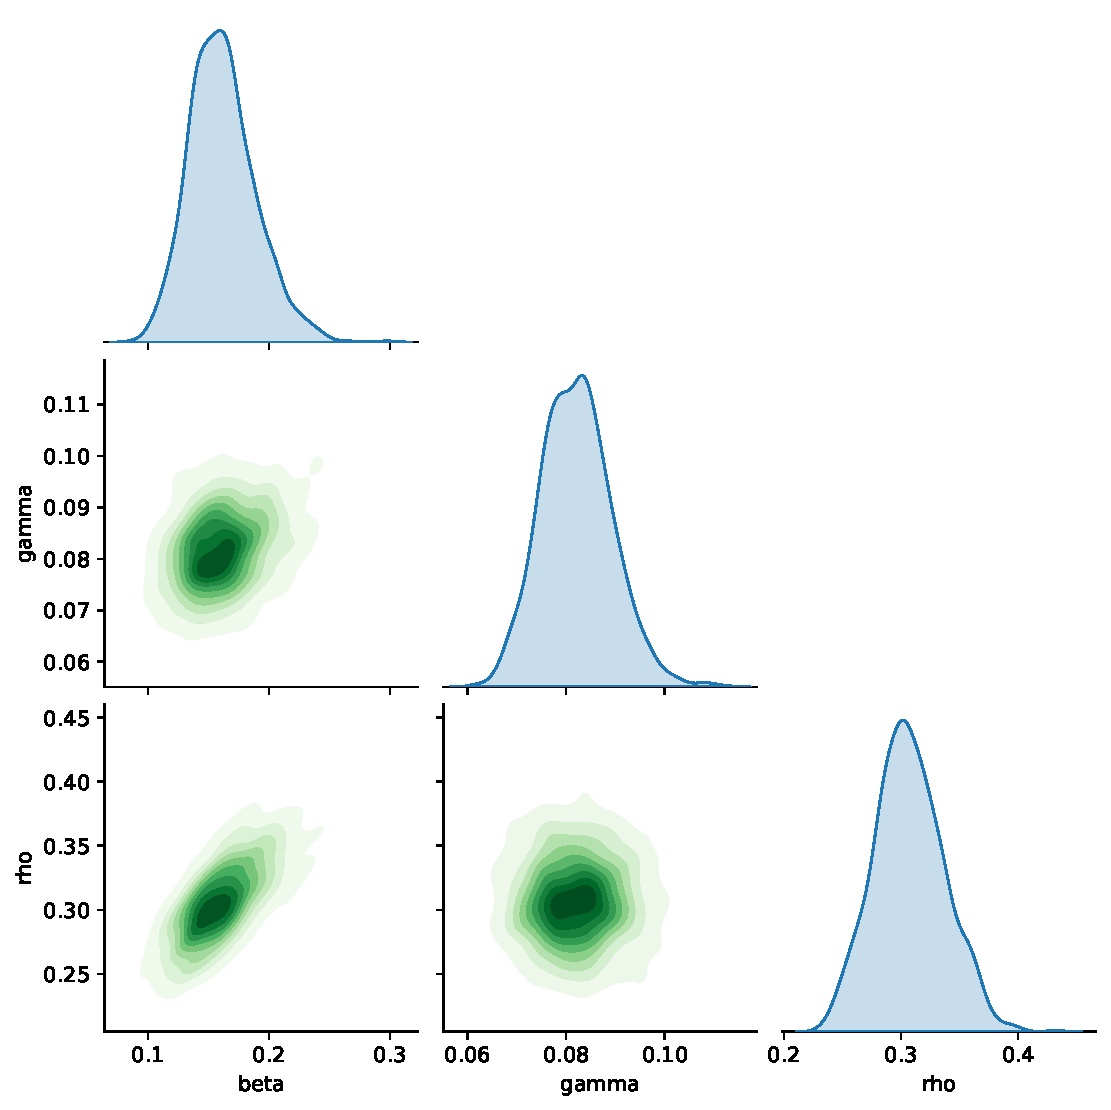
\includegraphics[width=\textwidth]{plots/smc_abc_pairplot_s5_mahalanobis.pdf}
        \caption{SMC Output (Raw)}
        \label{fig:reg_before}
    \end{subfigure}
    \hfill
    \begin{subfigure}[b]{0.48\textwidth}
        \centering
        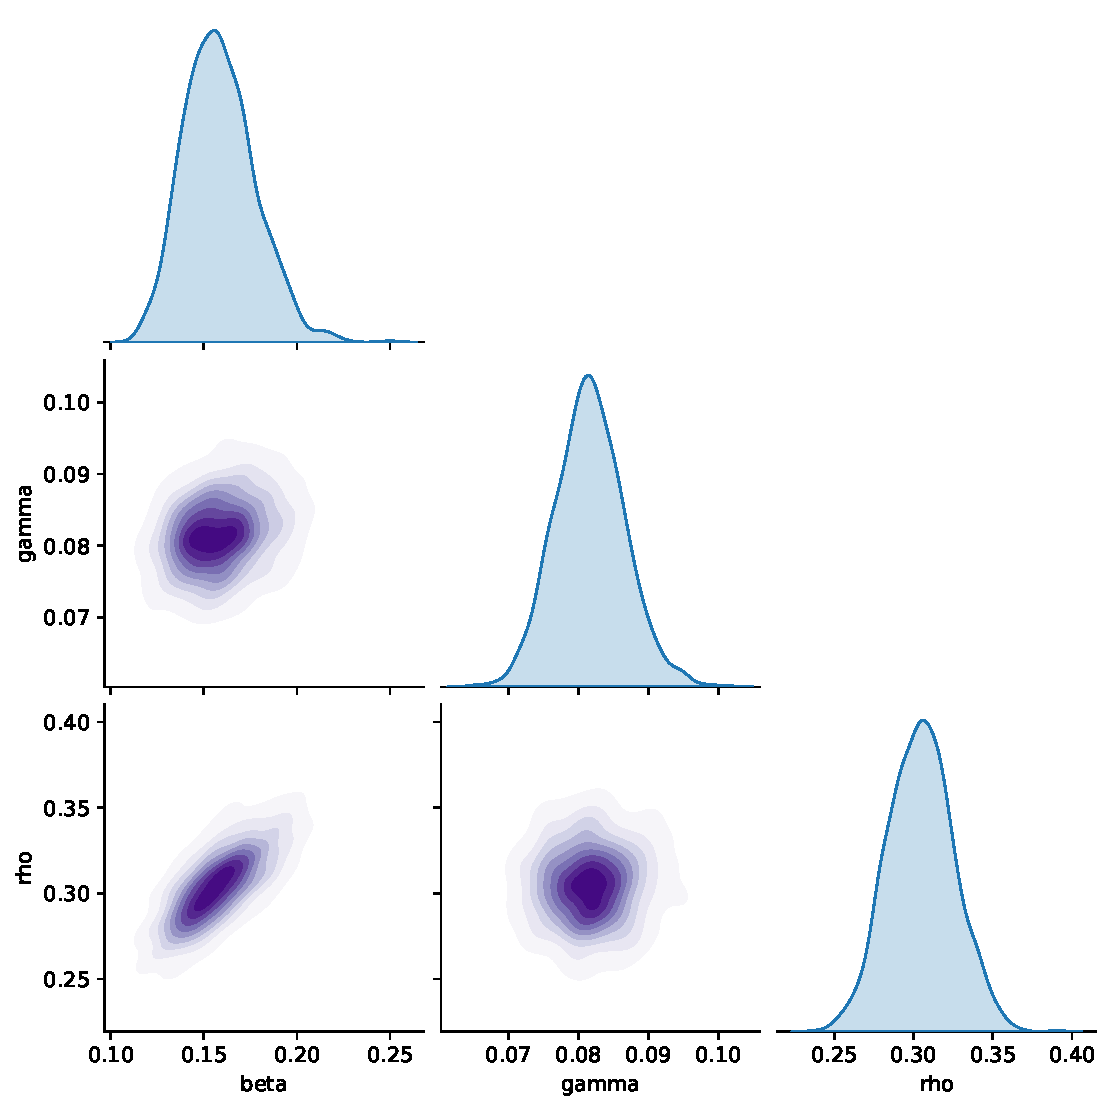
\includegraphics[width=\textwidth]{plots/smc_abc_pairplot_s5_regression_adjusted.pdf}
        \caption{Final (Regression Adjusted)}
        \label{fig:reg_after}
    \end{subfigure}
    \caption{Effect of Regression Adjustment.
This final step significantly reduces posterior variance and provides a highly concentrated estimate for all parameters.}
    \label{fig:reg_comparison}
\end{figure}

While Figure \ref{fig:reg_after} shows that a positive correlation between $\beta$ and $\rho$ persists, the extent of this ridge is drastically truncated compared to the baseline rejection sampling in Figure \ref{fig:abc_rejection_pairplot}.
This highly localized posterior mass demonstrates that our framework successfully resolves the severe equifinality, allowing for precise parameter identification despite the natural, structural trade-off between infection and rewiring inherent to the model.

\begin{table}[H]
\centering
\caption{Posterior Precision Improvement via Regression Adjustment}
\label{tab:regression_improvement}
\begin{tabular}{lcccc}
\toprule
Parameter & SD Reduction & 95\% CI Width Reduction \\
\midrule
Infection Rate ($\beta$) & 30.4\% & 33.8\% \\
Recovery Rate ($\gamma$) & 31.1\% & 29.7\% \\
Rewiring Rate ($\rho$)   & 30.4\% & 31.1\% \\
\bottomrule
\end{tabular}
\end{table}